\documentclass[a4paper]{article}
\usepackage[a4paper,margin=0mm]{geometry}
\usepackage{fontspec}
\usepackage{unicode-math}
\usepackage{tikz}
\usepackage[table]{xcolor}
\usepackage[absolute]{textpos}
\usepackage{enumitem}
\usepackage{array}
\usepackage{multirow}

\setmainfont{Libertinus Serif}
\setsansfont{Libertinus Sans}
\setmathfont{Libertinus Math}
\newfontfamily\trackedsans{Libertinus Sans}[LetterSpace=8.0]

\definecolor{accent}{HTML}{602785}
\definecolor{badge}{HTML}{B8A0C8}
\definecolor{ink}{HTML}{2A2E30}

\setlength{\TPHorizModule}{1mm}
\setlength{\TPVertModule}{1mm}
\setlength{\parindent}{0pt}
\pagestyle{empty}

% ---- Safe print margins: 16mm outer on both sides so bound/trimmed copies never
% clip problem text. Columns are 83mm wide with a 6mm gap on each side of the
% center rule (at x=105mm). ----
\newcommand{\LCOL}{16mm}
\newcommand{\RCOL}{111mm}
\newcommand{\COLW}{83mm}

% ---- Plain topic header: number chip + title, thin rule underneath. No band, no watermark. ----
\newcommand{\topicheader}[2]{%
\begin{textblock*}{194mm}(16mm,10mm)
\begin{tikzpicture}
\node[fill=accent,text=white,font=\sffamily\bfseries\fontsize{13}{13}\selectfont,
      minimum width=9mm,minimum height=9mm,inner sep=0pt] at (4.5mm,-4.5mm) {#1};
\node[font=\sffamily\bfseries\fontsize{15}{16}\selectfont,text=ink,anchor=west] at (12mm,-4.5mm) {#2};
\end{tikzpicture}
\end{textblock*}
\begin{textblock*}{194mm}(16mm,22.5mm)

\begin{tikzpicture}
\fill[accent] (0,0) rectangle (194mm,0.5mm);
\end{tikzpicture}
\end{textblock*}
}

\newcommand{\pagefooter}[1]{%
\begin{textblock*}{194mm}(8mm,286.41mm)
  
\begin{tikzpicture}
    \fill[accent] (0,0) rectangle (194mm,0.6mm);
  \end{tikzpicture}
\end{textblock*}
\begin{textblock*}{63.59mm}(8mm,288.27mm)
  {\sffamily\bfseries\color{accent}\fontsize{13}{16}\selectfont SAT 1200+}
\end{textblock*}
\begin{textblock*}{10mm}(188mm,288.27mm)
  \centering{\sffamily\color{accent}\fontsize{14}{16}\selectfont #1}
\end{textblock*}
}

% ---- Fixed-length vertical column rule: #1 = top y (mm), #2 = length (mm) ----
\newcommand{\colrule}[2]{%
\begin{textblock*}{1mm}(105mm,#1mm)
\begin{tikzpicture}
\draw[black!65,line width=0.5pt] (0,0) -- (0,#2mm);
\end{tikzpicture}
\end{textblock*}
}

\newcommand{\setkicker}[2]{%
{\sffamily\bfseries\fontsize{12}{14}\selectfont #1.}\ {\itshape\fontsize{11}{14}\selectfont\color{black!75} #2}\par\vspace{2mm}%
}

% ---- Small boxed problem number, reference-style. Plain \fbox -- stays flush with
% the text baseline instead of centering on it. ----
\setlength{\fboxsep}{1.4pt}
\setlength{\fboxrule}{0.5pt}
\newcommand{\pnum}[1]{\fcolorbox{ink}{white}{\sffamily\bfseries\fontsize{8}{8}\selectfont #1}~}

% ---- QR placeholder square + caption below ----
\newcommand{\qrbox}[1]{%
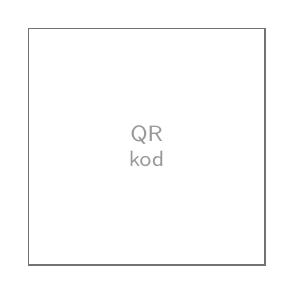
\begin{tikzpicture}
\draw[black!55,line width=0.6pt] (0,0) rectangle (30mm,30mm);
\node[black!40,font=\sffamily\fontsize{8}{9}\selectfont,align=center] at (15mm,15mm) {QR\\kod};
\end{tikzpicture}\\[1.5mm]
{\sffamily\fontsize{9}{11}\selectfont\color{black!70} #1}%
}

% ---- Answer-table styling: accent-colored grid, like the reference "Number | Answer" table ----
\arrayrulecolor{accent}
\setlength{\arrayrulewidth}{0.7pt}
\renewcommand{\arraystretch}{1.35}
\newcommand{\anstitle}[1]{{\sffamily\bfseries\color{accent}\fontsize{11}{13}\selectfont #1}\\[1.3mm]}

\begin{document}

% ================= PAGE 1: Set 1 | Set 2 =================
\topicheader{1}{Chiziqli tenglamalar va tengsizliklar}
\pagefooter{1}
\colrule{32}{238}
\mbox{}%

\begin{textblock*}{\COLW}(\LCOL,32mm)
{\fontsize{12}{15}\selectfont
\setkicker{1-to'plam}{Ko'p qadamli tenglamalar (Book 2 darajasida). $x$ ni toping.}

\noindent\pnum{1} $\dfrac{1}{2}(x+4)=x-1$\\[30mm]
\noindent\pnum{2} $3(x-2)=2(x+1)$\\[30mm]
\noindent\pnum{3} $\dfrac{2}{3}x+1=\dfrac{1}{3}x+5$\\[30mm]
\noindent\pnum{4} $5-2(x-3)=x+1$\\[30mm]
\noindent\pnum{5} $\dfrac{3}{4}(x-4)=2x-7$\\[30mm]
\noindent\pnum{6} $4(x+1)-3=2(x+5)$
}
\end{textblock*}

\begin{textblock*}{\COLW}(\RCOL,32mm)
{\fontsize{12}{15}\selectfont
\setkicker{2-to'plam}{"Nima so'ralyapti" qopqoni -- tenglamani yeching, lekin aynan so'ralgan qiymatni bering, shunchaki $x$ ni emas.}

\noindent\pnum{1} Agar $3x+5=20$ bo'lsa, $6x+10$ nechiga teng?\\[22mm]
\noindent\pnum{2} Agar $2(x-3)=10$ bo'lsa, $x-3$ nechiga teng?\\[22mm]
\noindent\pnum{3} Agar $4x-7=9$ bo'lsa, $2x$ nechiga teng?\\[22mm]
\noindent\pnum{4} Agar $\dfrac{x+2}{3}=5$ bo'lsa, $x+2$ nechiga teng?\\[22mm]
\noindent\pnum{5} Agar $5x+1=26$ bo'lsa, $10x+2$ nechiga teng?\\[22mm]
\noindent\pnum{6} Agar $3(2x+1)=21$ bo'lsa, $2x+1$ nechiga teng?
}
\end{textblock*}

\clearpage

% ================= PAGE 2: Set 3 | Set 4 =================
\topicheader{1}{Chiziqli tenglamalar va tengsizliklar}
\pagefooter{2}
\colrule{32}{238}
\mbox{}%

\begin{textblock*}{\COLW}(\LCOL,32mm)
{\fontsize{12}{15}\selectfont
\setkicker{3-to'plam}{Tengsizliklar -- ishora almashinuviga e'tibor bering. $x$ ni toping.}

\noindent\pnum{1} $2x+3<11$\\[30mm]
\noindent\pnum{2} $-4x+1\ge13$\\[30mm]
\noindent\pnum{3} $5-x\le8$\\[30mm]
\noindent\pnum{4} $\dfrac{1}{2}x-3>1$\\[30mm]
\noindent\pnum{5} $-3(x-2)<9$\\[30mm]
\noindent\pnum{6} $7-3x\ge-5$
}
\end{textblock*}

\begin{textblock*}{\COLW}(\RCOL,32mm)
{\fontsize{12}{15}\selectfont
\setkicker{4-to'plam}{Qo'shma tengsizliklar. $x$ ni toping.}

\noindent\pnum{1} $-2<x+3\le7$\\[30mm]
\noindent\pnum{2} $3x-1<-4$ yoki $3x-1>8$\\[30mm]
\noindent\pnum{3} $-5\le2x+1<9$\\[30mm]
\noindent\pnum{4} $x-4<-6$ yoki $x-4>2$\\[30mm]
\noindent\pnum{5} $-1<\dfrac{x+1}{2}\le3$\\[30mm]
\noindent\pnum{6} $2x+3<1$ yoki $2x+3>9$
}
\end{textblock*}

\clearpage

% ================= PAGE 3: Set 5 | Set 6 (spot the error) =================
\topicheader{1}{Chiziqli tenglamalar va tengsizliklar}
\pagefooter{3}
\colrule{32}{238}
\mbox{}%

\begin{textblock*}{\COLW}(\LCOL,32mm)
{\fontsize{11.5}{14.5}\selectfont
\setkicker{5-to'plam}{So'zlardan tengsizlikka o'tkazing, so'ng yeching.}

\noindent\pnum{1} Biror son 5 ga oshirilsa, natija kamida 12 bo'ladi. (Sonni toping.)\\[20mm]
\noindent\pnum{2} Biror sonning uch barobari 21 dan oshmaydi.\\[20mm]
\noindent\pnum{3} Biror son 4 ga kamaytirilsa, natija 10 dan kichik.\\[20mm]
\noindent\pnum{4} Biror sonning ikki barobari, 3 ga kamaytirilganda, kamida 7.\\[20mm]
\noindent\pnum{5} Biror son kamida $-1$ va ko'pi bilan $5$. (Faqat qo'shma tengsizlikni yozing -- yechish shart emas.)\\[20mm]
\noindent\pnum{6} Sonning ikki barobaridan besh kam -- 15 dan oshmaydi. Sonning eng katta butun qiymati nechiga teng?
}
\end{textblock*}

\begin{textblock*}{\COLW}(\RCOL,32mm)
{\fontsize{11}{14}\selectfont
\setkicker{6-to'plam}{Xatoni toping -- buzilgan qadamni ayting, to'g'ri javobni bering.}

\noindent\pnum{1} $-2x>8$ ifodasida ko'rsatilgan yechimda xato bor:\\[1mm]
\hspace*{7mm}\textit{``Ikkala tomonni $-2$ ga bo'ling: $x>-4$.''}\\[2mm]
\hspace*{7mm}Xato va to'g'ri javob: \makebox[52mm]{\dotfill}\\[8mm]

\noindent\pnum{2} $x-5>2$ ifodasida ko'rsatilgan yechimda xato bor:\\[1mm]
\hspace*{7mm}\textit{``Manfiy son bor, shuning uchun ishora almashadi: $x<7$.''}\\[2mm]
\hspace*{7mm}Xato va to'g'ri javob: \makebox[52mm]{\dotfill}\\[8mm]

\noindent\pnum{3} Agar $4x-1=15$ bo'lsa, $4x$ nechiga teng ifodasida xato bor:\\[1mm]
\hspace*{7mm}\textit{``$x=4$, demak javob $4$.''}\\[2mm]
\hspace*{7mm}Xato va to'g'ri javob: \makebox[52mm]{\dotfill}\\[8mm]

\noindent\pnum{4} $-2(x-3)<10$ ifodasida ko'rsatilgan yechimda xato bor:\\[1mm]
\hspace*{7mm}\textit{``Taqsimlang: $-2x-6<10$, demak $x>-8$.''}\\[2mm]
\hspace*{7mm}Xato va to'g'ri javob: \makebox[52mm]{\dotfill}\\[8mm]

\noindent\pnum{5} $-4<2x<8$ ifodasida ko'rsatilgan yechimda xato bor:\\[1mm]
\hspace*{7mm}\textit{``O'rta va o'ng tomonni 2 ga bo'ling: $-4<x<4$.''}\\[2mm]
\hspace*{7mm}Xato va to'g'ri javob: \makebox[52mm]{\dotfill}
}
\end{textblock*}

\clearpage

% ================= PAGE 4: Set 7 (bonus) -- own page; answers follow on a fresh page =================
\topicheader{1}{Chiziqli tenglamalar va tengsizliklar}
\pagefooter{4}
\colrule{32}{238}
\mbox{}%

\begin{textblock*}{\COLW}(\LCOL,32mm)
{\fontsize{11.5}{14.5}\selectfont
\setkicker{7-to'plam}{Bonus / qiyin -- eng qiyin topshiriqlar.}

\noindent\pnum{1} Agar $\dfrac{2}{3}(x-3)=x-5$ bo'lsa, $x$ ni, so'ng $3x$ ni toping.\\[32mm]
\noindent\pnum{2} $-5<3x+1\le10$ ni yeching. Qo'shma tengsizlikni yozing, so'ng shartni qanoatlantiruvchi eng kichik butun $x$ qiymatini toping.\\[32mm]
\noindent\pnum{3} Yetti minus sonning ikki barobari kamida $-3$. Sonning eng katta qiymati nechiga teng?\\[32mm]
\noindent\pnum{4} $4(x-1)-2x=3(x+2)-10$ ni $x$ uchun yeching, so'ng $x+2$ ni toping.\\[32mm]
\noindent\pnum{5} $-6\le-2(x-1)<4$ ni yeching.
}
\end{textblock*}

\clearpage

% ================= PAGE 5: Javoblar -- full-page answer tables, own page always =================
\topicheader{1}{Chiziqli tenglamalar va tengsizliklar}
\pagefooter{5}
\mbox{}%

\begin{textblock*}{194mm}(16mm,30mm)
{\bfseries\itshape\color{accent}\fontsize{19}{21}\selectfont\centering Javoblar\par}
\end{textblock*}

\begin{textblock*}{194mm}(16mm,44mm)
{\fontsize{9.5}{12}\selectfont
\centering
\renewcommand{\arraystretch}{1.3}
\begin{tabular}{|>{\centering\arraybackslash}p{26mm}|>{\centering\arraybackslash}p{9mm}|>{\centering\arraybackslash}p{32mm}|>{\centering\arraybackslash}p{9mm}|>{\centering\arraybackslash}p{32mm}|}
\hline
\rowcolor{badge!55}\textbf{To'plam} & \textbf{\#} & \textbf{Javob} & \textbf{\#} & \textbf{Javob}\\
\hline
\multirow{3}{26mm}{\centering 1-to'plam} & 1 & $x=6$ & 2 & $x=8$\\\cline{2-5}
 & 3 & $x=12$ & 4 & $x=\tfrac{10}{3}$\\\cline{2-5}
 & 5 & $x=\tfrac{16}{5}$ & 6 & $x=\tfrac{9}{2}$\\\hline
\multirow{3}{26mm}{\centering 2-to'plam} & 1 & $40$ & 2 & $5$\\\cline{2-5}
 & 3 & $8$ & 4 & $15$\\\cline{2-5}
 & 5 & $52$ & 6 & $7$\\\hline
\multirow{3}{26mm}{\centering 3-to'plam} & 1 & $x<4$ & 2 & $x\le-3$\\\cline{2-5}
 & 3 & $x\ge-3$ & 4 & $x>8$\\\cline{2-5}
 & 5 & $x>-1$ & 6 & $x\le4$\\\hline
\multirow{3}{26mm}{\centering 4-to'plam} & 1 & $-5<x\le4$ & 2 & $x<-1$ yoki $x>3$\\\cline{2-5}
 & 3 & $-3\le x<4$ & 4 & $x<-2$ yoki $x>6$\\\cline{2-5}
 & 5 & $-3<x\le5$ & 6 & $x<-1$ yoki $x>3$\\\hline
\multirow{6}{26mm}{\centering 5-to'plam} & \multicolumn{4}{p{84mm}|}{1.\ $x+5\ge12 \Rightarrow x\ge7$}\\\cline{2-5}
 & \multicolumn{4}{p{84mm}|}{2.\ $3x\le21 \Rightarrow x\le7$}\\\cline{2-5}
 & \multicolumn{4}{p{84mm}|}{3.\ $x-4<10 \Rightarrow x<14$}\\\cline{2-5}
 & \multicolumn{4}{p{84mm}|}{4.\ $2x-3\ge7 \Rightarrow x\ge5$}\\\cline{2-5}
 & \multicolumn{4}{p{84mm}|}{5.\ $-1\le x\le5$}\\\cline{2-5}
 & \multicolumn{4}{p{84mm}|}{6.\ $2x-5\le15 \Rightarrow x\le10$, eng katta butun $=10$}\\\hline
\multirow{5}{26mm}{\centering 6-to'plam} & \multicolumn{4}{p{84mm}|}{1.\ Xato -- manfiyga bo'lganda ishora almashishi kerak, lekin yo'nalish teskari ko'rsatilgan. To'g'ri: $x<-4$.}\\\cline{2-5}
 & \multicolumn{4}{p{84mm}|}{2.\ Xato -- manfiyga ko'paytirish/bo'lish bo'lmagan (faqat ayirish), ishora almashmasligi kerak. To'g'ri: $x>7$.}\\\cline{2-5}
 & \multicolumn{4}{p{84mm}|}{3.\ Xato -- $4x$ o'rniga $x$ berilgan. To'g'ri: $x=4$, demak $4x=16$.}\\\cline{2-5}
 & \multicolumn{4}{p{84mm}|}{4.\ Xato -- $-2\times(-3)$ ni $-6$ deb taqsimlagan, $+6$ bo'lishi kerak edi. To'g'ri: $-2x+6<10 \Rightarrow x>-2$.}\\\cline{2-5}
 & \multicolumn{4}{p{84mm}|}{5.\ Xato -- o'rta va o'ng tomon 2 ga bo'lingan, lekin $-4$ bo'linmay qolgan. To'g'ri: $-2<x<4$.}\\\hline
\multirow{5}{26mm}{\centering 7-to'plam} & \multicolumn{4}{p{84mm}|}{1.\ $x=9$, $3x=27$}\\\cline{2-5}
 & \multicolumn{4}{p{84mm}|}{2.\ $-2<x\le3$, eng kichik butun $=-1$}\\\cline{2-5}
 & \multicolumn{4}{p{84mm}|}{3.\ $x\le5$, eng katta qiymat $=5$}\\\cline{2-5}
 & \multicolumn{4}{p{84mm}|}{4.\ $x=0$, $x+2=2$}\\\cline{2-5}
 & \multicolumn{4}{p{84mm}|}{5.\ $-1<x\le4$}\\\hline
\end{tabular}
}
\end{textblock*}

\begin{textblock*}{194mm}(16mm,232mm)
\centering
{\sffamily\fontsize{9.5}{11.5}\selectfont\color{black!70} Video yechimlar va qo'shimcha testlar uchun quyidagi QR kodlarni skanerlang:}\\[4mm]
\begin{minipage}[t]{32mm}\centering\qrbox{YouTube}\end{minipage}%
\hspace{16mm}%
\begin{minipage}[t]{32mm}\centering\qrbox{Telegram}\end{minipage}
\end{textblock*}

\end{document}
